\section{MAŠININIO MOKYMOSI APŽVALGA}
\label{darbu_apzvalga}

Mašininis mokymasis (angl. \textit{machine learning}) yra dirbtinio intelekto šaka, kurios tyrėjai siekia įgalinti kompiuterius tobulinti savo elgseną (mokytis) empirinių duomenų atžvilgiu \cite{duda2001pattern}. Pagal tai, kokie yra turimi empiriniai duomenys, mašininis mokymasis yra skirstomas į mokymąsi su mokytoju (angl. \textit{supervised learning}) ir mokymąsi be mokytojo (angl. \textit{unsupervised learning}).

Biomedicinos kontekste mašininiu mokymusi siekiama atrasti dėsningumus turimuose duomenyse ir išmokti juos panaudoti. Biomedicininius duomenis sudaro mėginių aibė apibūdinama daugeliu matų. Mėginiai priklauso kelioms grupėms (klasėms), pvz., sergančių ir kontrolinių pacientų grupėms. Mašininio mokymosi su mokytoju tikslas -- išmokti funkciją atskiriančią mėginius į grupes ir pritaikyti ją dar nematytiems mėginiams. Mokymosi be mokytojo tikslas -- nustatyti mėginių grupes pagal turimus duomenis.

 Toliau šiame skyriuje apžvelgiami mašininio mokymosi teorijos pagrindai, kurie yra būtini analizuojant daugiamačius biomedicininius duomenis: mokymasis su mokytoju, mokymasis be mokytojo, atraminių vektorių klasifikatoriai, \textit{Random Forest} klasifikatorius.

\subsection{Mokymasis su mokytoju}

Žmonės mokosi iš patirties, tačiau, skirtingai nei žmonės, kompiuteriai patirties neturi, todėl kompiuteriai turi mokytis iš patyrimą apibūdinančių duomenų -- mokymosi duomenų (angl. \textit{training data}). Mokymosi su mokytoju tikslas yra sukonstruoti funkciją, kuri galėtų būti naudojama nuspėti testavimo duomenų (angl. \textit{testing data}) charakteristikų reikšmes pagal mokymosi duomenis. Mokytojo vaidmenį atlieka mokymosi duomenys, kurių spėjamų charakteristikų reikšmės yra iš anksto žinomos. Pagal tai, kokias charakteristikas bandoma nuspėti mokymasis su mokytoju yra skirstomas į dvi rūšis:
\begin{enumerate}
  \item Klasifikavimas (angl. \textit{classification}) -- pagal mokymosi duomenų nepriklausomus kintamuosius bandoma nuspėti kokybinius (kategorinės reikšmės) priklausomus kintamuosius.
  \item Regresinė analizė (angl. \textit{regression}) -- pagal mokymosi duomenų nepriklausomus kintamuosius bandoma nuspėti kiekybinius (tolydinės reikšmės) priklausomus kintamuosius.
\end{enumerate} 

%% JG: Pateik vizualų klasifikavimo pavyzdį iliustruojanti visus 3 etapus.
%% DJ: Vizualų, ta prasme su paveiksliukais ar ir tas pavyzdys su paštu pakankamai vaizdingas?
%% JG: Reikia kitaip struktūrizuoti šitą skyrių: 
% +Pradžioj pasakyk, kad yra klasifikavimas ir regresija ir po
%  sakinįÂ kiekvienam.
% +Tada aptark klasifikavimą ir pateik pavyzdį. 
% +Tada pateik regresijos pavyzdį.
% +Tada parašyk, kad šiame darbe studijuojama klasifikavimo problema.

\subsubsection{Klasifikavimas}

Mašinininio mokymosi kontekste klasifikavimu yra vadinama problema, kai naudojantis mokymosi duomenis reikia išmokti nustatyti, kuriai klasei priklauso mėginys. Klasifikavimo procesas trimis etapais pavaizduoti ~\ref{fig:classification_process} pav. srautų diagramoje. Klasifikavimo etapai:
\begin{enumerate}
 \item Visa mokymosi duomenų aibė yra atsitiktinai padalinama į dvi nepersidengiančias aibes: treniravimos duomenys (pvz., 90\% visų mokymosi duomenų) ir testavimo duomenys(pvz., likę 10\%);
 \item Pagal turimus treniravimosi duomenis yra atrenkami informatyviausi matai, pvz., naudojant Relief metodą. Remiantis atrinktaisiais matais yra konstruojamas klasifikatorius - funkcija, pagal kurią nematyti mėginiai bus priskirti vienai iš klasių.
 \item Sukonstruotu klasifikatoriumi testavimo duomenys yra suskirstomi į klases. Pagal tai, kiek mėginių klasifikatorius priskyrė teisingoms klasėms yra vertinama klasifikatoriaus tikslumas. Klasifikatorius validuojamas naudojant tokius metodus kaip kryžminis patikrinimas (angl. \textit{cross validation})
\end{enumerate}

Dirbant su biomedicininiais duomenimis tipinė užduotis yra pagal paciento mėginį apibūdinančius matus sukonstruoti klasifikatorių, kuris bandys nuspėti, kuriai pacientų klasei -- sergančiųjų ar sveikųjų -- priklauso tiriamasis mėginys.
\begin{figure}
 \centering
 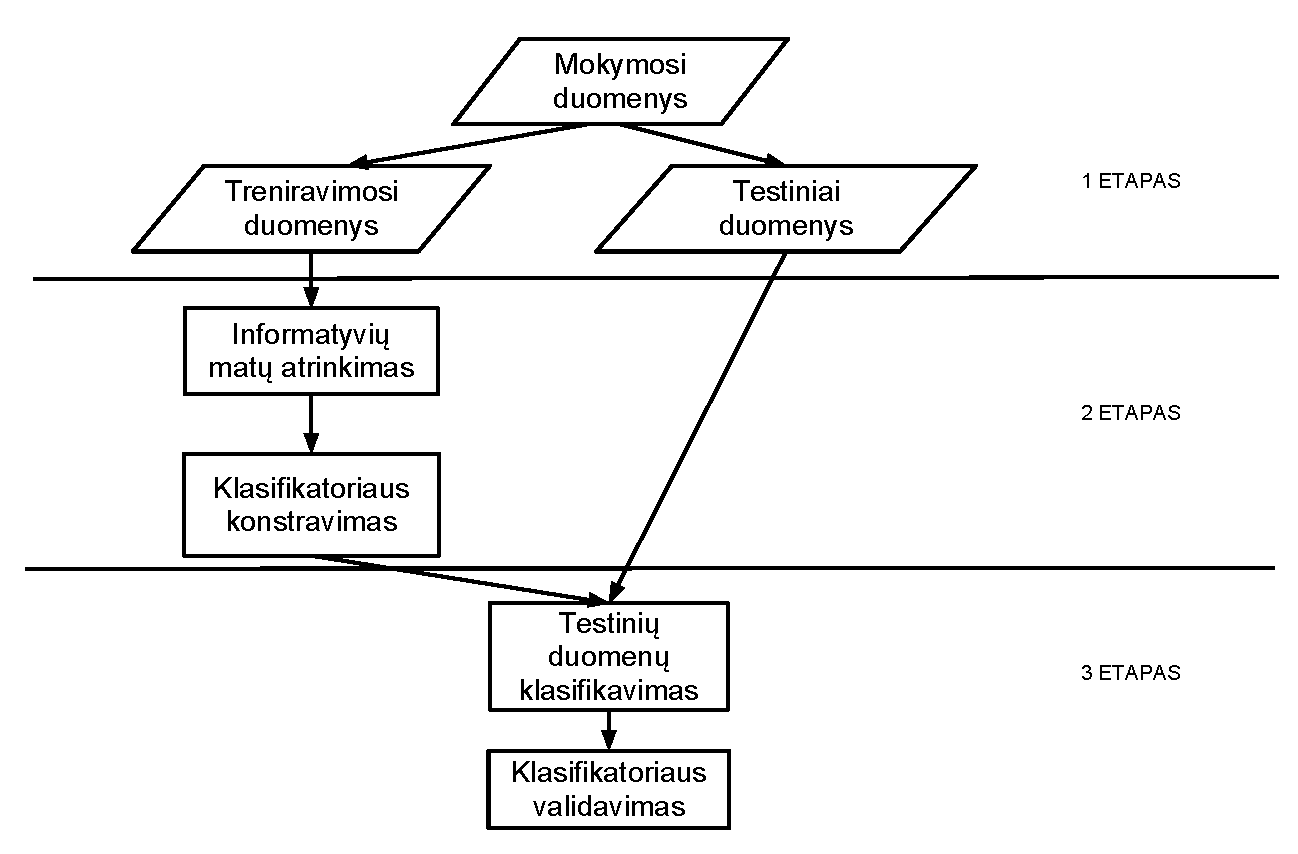
\includegraphics[width=\textwidth]{images/classification_process.pdf}
 \caption{Klasifikavimo srautų diagrama su paaiškinimais.}
 \label{fig:classification_process}
\end{figure}
Klasifikavimą galima vertinti pagal:
\begin{itemize}
 \item Klasifikavimo tikslumą (angl. \textit{accuracy}) -- santykį tarp teisingai suklasifikuotų mėginių ir visų mėginių;
 \item Klasifikavimo nuostolius (angl. \textit{error rate}) -- santykį tarp neteisingai suklasifikuotų mėginių ir visų mėginių;
 \item ROC (angl. \textit{receiver operating characteristic}, ROC) kreivę -- grafikas, rodantis klasifikatoriaus jautrumą ir specifiškumą. Grafiko abscisių ašyje atidedamos klasifikatoriaus specifiškumo (angl. \textit{false positive}) reikšmės, o ordinačių ašyje jautrumo (angl. \textit{true positive}) reikšmės.
\end{itemize}

\paragraph{Klasifikatoriaus validavimas kryžminio patikrinimo metodu}

Naudojant kryžminio patikrinimo (angl. \textit{cross-validation}) metodą, daug kartų sudaromos skirtingos treniravimosi ir testavimo mėginių imtys. Taikant atskirą šio metodo variantą, kryžminį patikrinimą paliekant vieną mėginį (angl. \textit{leave-one-out cross-validation}), iš mokymosi duomenų išimamas vienas (testavimo) mėginys, o su likusiais apmokomas klasifikatorius, kuris klasifikuoja išbrauktąjį mėginį. Procesas tęsiamas tol, kol suklasifikuojami visi mėginiai. Kitais kryžminio patikrinimo metodo variantais iš treniravimosi mėginių yra išimama po keletą mėginių. Pagal tai, kiek testavimo mėginių klasifikatorius priskyrė klaidingai kategorijai, yra nustatoma vidutinė klaidingo klasifikavimo tikimybė. Šiuo metodu gauti įverčiai pasižymi dideliu klasifikavimo rezultatų variabilumu \cite{braga2004cross}.

\paragraph{Klasifikatoriaus validavimas įkelčių metodu}

Naudojant įkelčių metodą, iš $N$ dydžio mėginių aibės yra paimama tokio pačio dydžio atsitiktinių mėginių imtis su pasikartojimais, kuri vadinama įkelties treniravimosi imtimi. Į šią imtį nepaimti mėginiai yra priskiriami testavimo imčiai. Naudojant įkelties treniravimosi mėginių imtį yra apmokomas klasifikatorius, kuris klasifikuoja testavimo imtį. Procesą kartojant gaunama klasifikavimo nuostolių įverčių imtis. Šios imties vidurkis yra vidutinis klasifikavimo nuostolio įvertis. Dažniausiai naudojamas ,,0.623 įkelčių`` (angl. \textit{0.623\footnote{0.623 yra tikimybė mėginiui būti įtrauktam į treniravimosi imtį.} bootstrap}) metodas. Šiuo metodu gautas vidutinio klasifikavimo nuostolio įvertis pasižymi mažu variabilumu \cite{michie1994machine}.

\subsubsection{Regresinė analizė}

Mašininio mokymosi kontekste regresine analize yra vadinama problema, kai pagal patirtį apibūdinančius duomenis reikia nustatyti kiekybines duomenų charakteristikas. Regresinė analizė naudoja standartinius statistinius metodus, tokius kaip mažiausių kvadratų metodas (angl. \textit{least squares}). Regresinė analizė dažniausiai naudojama įvertinti (ang. \textit{forecast}) ateities duomenų vertes bei interpoliacijai -- tikėtinos reikšmės tarp keletos taškų įvertinimui. 

Dirbant su biomedicininiais duomenimis regresinė analizė taikoma nustatant, pvz., mėginio vėžio stadiją. Šiame darbe pagrindinis dėmesys skiriamas klasifikavimui. Daugiau informacijos apie regresiją galima rasti \cite{gelman2007data}.

\subsubsection{Atraminių vektorių klasifikatoriai}

Atraminių vektorių klasifikatoriai (angl. \textit{support vector machines}, SVM) - tai mokymosi su mokytoju algoritmas, kuris gali būti taikomas tiek klasifikavimui, tiek regresinei analizei \cite{vapnik2000nature}. Atraminių vektorių klasifikatorių algoritmo tikslas yra mėginių erdvėje orientuoti atskiriančiąją hiperplokštumą, galimai pašalinant triukšmą bei išimtis (angl. \textit{outlier}), tokiu būdu, kad atstumas tarp jos ir atraminių vektorių būtų didžiausias \cite{cortes1995support}. Atraminiais vektoriais (angl. \textit{support vectors}) yra vadinami abiejų klasių mėginiai esantys arčiausiai atskiriančiosios hiperplokštumos (angl. \textit{decision boundary}).

\paragraph{Tiesiškai atskiriami duomenys}

Tarkime, kad turime $L$ mokymosi mėginių, kurių kiekvienas mėginys $x_i$ turi $D$ matų ir priklauso vienai iš dviejų klasių $y_i=-1$ arba $y_i=+1$. Taigi turime mokymosi duomenis, kurių pavidalas yra:
\begin{equation}
 \{x_i, y_i\}, kur\; i=1..L, y_i \in \{-1,1\}, x \in \Re^D
\end{equation}
Kai duomenys yra tiesiškai atskiriami, galima nupiešti tiesę plokštumoje $x_1$ ir $x_2$, kuri atskiria dvi klases, kai $D=2$ ir hiperplokštumą erdvėje $x_1, x_2,...x_D$, kai $D > 2$. Atskiriančioji tiesė pavaizduota \ref{fig:support_vector_machines} pav. Hiperplokštuma apibrėžta $w\cdot x_i + b = 0$, kur $w$ -- hiperplokštumos normalės vektorius, $\frac{b}{||w||}$ -- statmens einančio nuo hiperplokštumos iki koordinačių pradžios taško ilgis (sisteminis nuokrypis (angl. \textit{bias})).
\begin{figure}
 \centering
 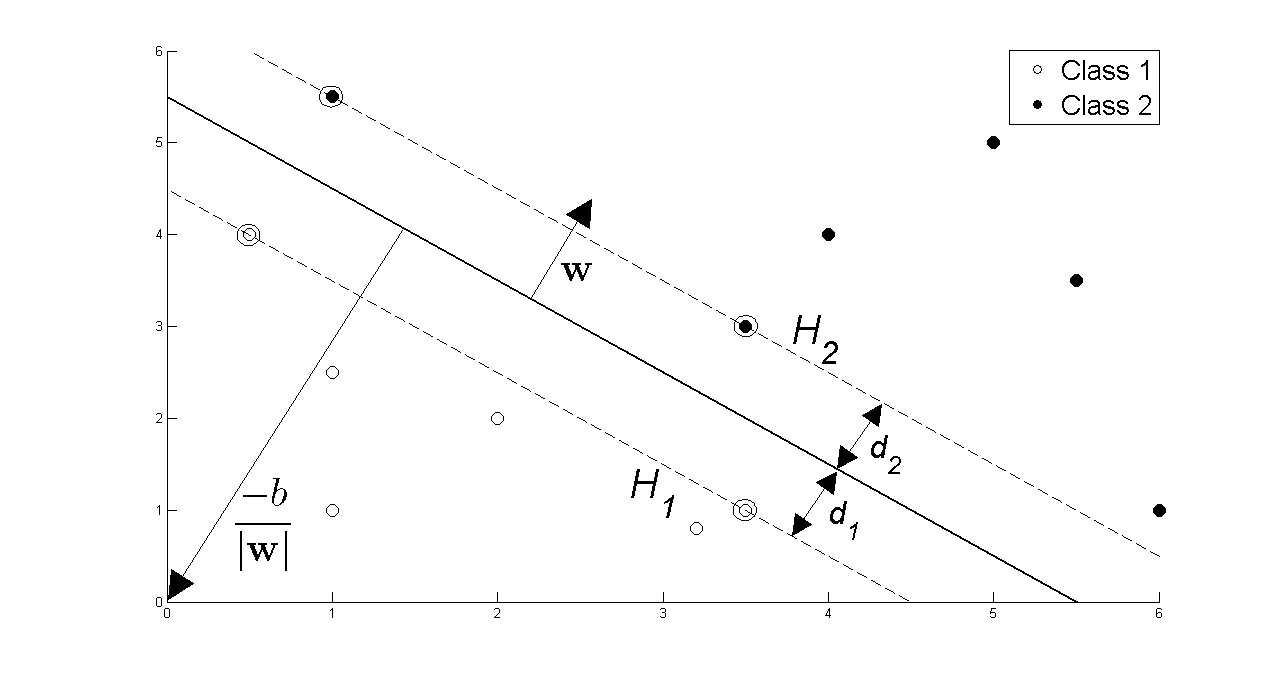
\includegraphics[width=.7\textwidth]{images/support_vector_machines.jpg}
 \caption{Atskiriančiosioji tiesė nubrėžta plokštumoje, kurioje pavaizduoti tiesiškai atskiriami duomenys \cite{fletcher2009support}.}
 \label{fig:support_vector_machines}
\end{figure}

 Taigi, atraminių vektorių klasifikatorių sukūrimas yra parametrų $w$ ir $b$, tenkinančių minėtas sąlygas, radimas. Klasifikavimo taisyklę $f$ testavimo duomenims $X$ apibrėžiama formule:
\begin{equation}
 \label{svm_separable}
 f(X) = sign(w^T X + b),
\end{equation}
kur $w^T$ yra transponuotas matų svorių vektorius.

\paragraph{Tiesiškai neatskiriami duomenys}

Kai duomenys yra tiesiškai neatskiriami, matų erdvės transformavimas gali padėti duomenis padaryti tiesiškai atskiriamais. Branduolio metodai (angl. \textit{kernel methods}) transformuoja matų erdvę taip, kad jie tampa tiesiškai atskiriami \cite{aizerman1964theoretical}. Tokios transformacijos pavyzdys pateiktas \ref{fig:matu_erdves_transformavimas} pav\footnote{Nuoroda į šaltinį: http://omega.albany.edu:8008/machine-learning-dir/notes-dir/ker1/ker1-l.html}.
\begin{figure}
 \centering
 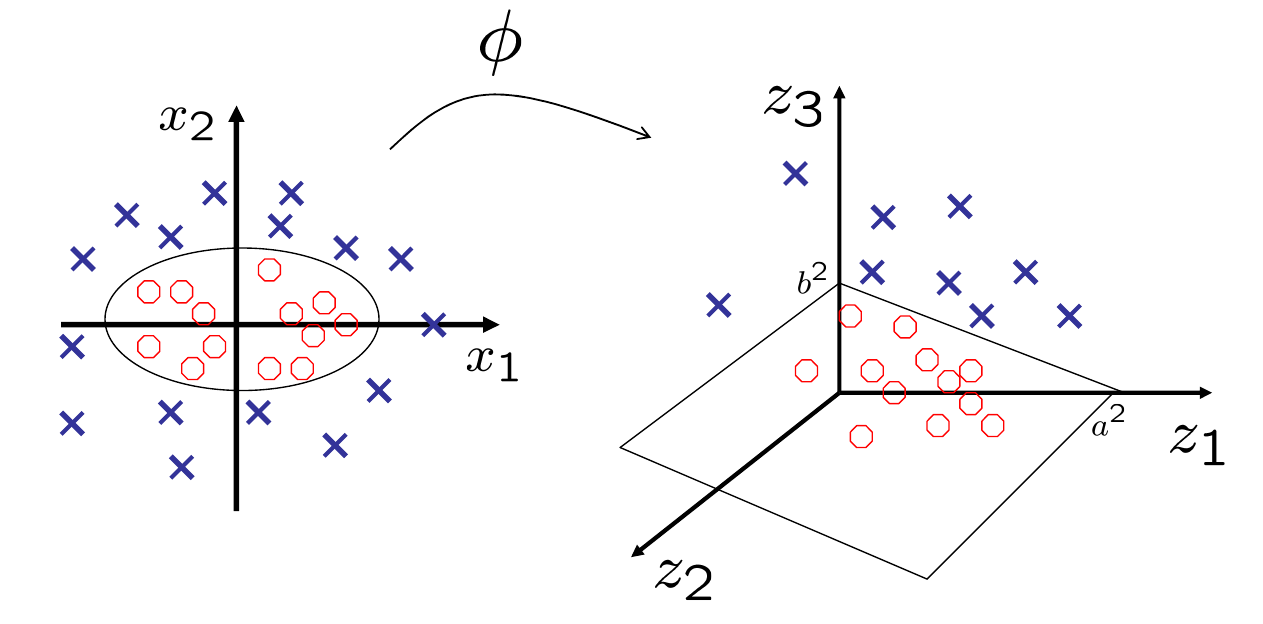
\includegraphics[width=.7\textwidth]{images/matu_erdves_transformavimas.png}
 \caption{Tiesiškai neatskiriamos matų erdvės transformavimas į tiesiškai atskiriamą.}
 \label{fig:matu_erdves_transformavimas}
\end{figure}

Branduoliu (angl. \textit{kernel}) vadinama funkcija:
\begin{equation}
 \label{kernel}
 K(X, Y) = \langle \phi(X)^T \cdot \phi(Y) \rangle
\end{equation}
Branduolio funkcija naudojama tiesiškai neatskiriamų duomenų erdvės projektavimui į kitą erdvę, kurioje duomenys būtų tiesiškai atskiriami. 
Branduolio savybė, kai jį galima išreikšti funkcija nuo pradinių kintamųjų skaliarinės sandaugos, vadinama ,,branduolio gudrybe`` (angl. \textit{kernel trick}). ,,Branduolio gudrybė`` dažniausiai naudojama norint tiesinį metodą paversti netiesiniu. 

Pavyzdžiui, branduolys yra $K(X, Y)=\langle X \cdot Y \rangle ^ 2$, o $\phi(x_1, x_2)=(x_1^2, \sqrt{2}x_1x_2, x_2^2)^2$ transformuoja matų erdvę iš $R^2$ į $R^3$. Turime mėginius $X=(x_1, x_2),\; Y=(y_1, y_2)$. Branduolį taikome mėginiams $K(X, Y) = \langle X \cdot Y \rangle ^ 2 = \langle x_1y_1 + x_2y_2\rangle ^ 2 = \langle x_1^2y_1^2 + 2x_1y_1x_2y_2 + x_2^2y_2^2 \rangle = \langle (x_1^2, \sqrt{2}x_1x_2, x_2^2) \cdot (y_1^2, \sqrt{2}y_1y_2, y_2^2) \rangle = \langle \phi(X) \cdot \phi(Y) \rangle$.

Atraminių vektorių klasifikatorių algoritmo naudojimas dirbant su biomedicininiais duomenimis populiarus, nes jis demonstruoja gerus rezultatus, kai turima maža daugiamačių mokymosi duomenų aibė. 

%% JG: cituoti turi originalų darbą:
%% JG: C. Cortes and V. Vapnik, Support-Vector Networks, Machine Learning, 20(3):273-297, September 1995
%% JG: Vladimir N. Vapnik. The Nature of Statistical Learning Theory. Springer, New York, 1995

%SVM is a type of machine learning algorithm derived from statistical learning
%[theory](http://download.oracle.com/docs/cd/B14117_01/text.101/b10729/classify.htm).

%% JG: nepamiršksio daugiamatiškumo erdvę, o ten juos galima atskirti tiesiškai.

\subsubsection{\textit{Random Forest} klasifikatorius}

\textit{Random Forrest} klasifikatorius yra kombinuotojo mokymosi algoritmas, kuris sukuria keletą klasifikavimo medžių (angl. \textit{decision tree}) \cite{DBLP:books/mk/HanK2000}, kurie  nepriklausomai klasifikuoja mėginius, ir daugumos balsavimo (angl. \textit{majority voting}) būdu yra skelbiamas galutinis klasifikavimo rezultatas \cite{breiman1984classification}. Kiekvienas klasifikavimo medis yra konstruojamas pagal algoritmą nr. \ref{random_forest_algorithm}.
\begin{algorithm}
 \caption{\textit{Random Forest} klasifikavimo medžių konstravimas}
 \label{random_forest_algorithm}
 \begin{enumerate}
  \item Turima $N$ mėginių, kurie turi $M$ matų;
  \item Pasirenkamas $m$ matų, kurie bus naudojami klasifikavimo medžių kūrimui; $m << M$;
  \item Sudaroma treniravimosi mėginių aibė, $n$ kartų pasirenkant mėginius su pasikartojimais iš visų $N$ mėginių. Visi nepasirinkti mėginiai paliekami klasifikatoriaus testavimui; 
  \item Kiekvienam medžio mazgui atsitiktinai pasirenkama $m$ matų, kuries sudarys sąlygą tam mazgui. Randamas geriausia atskyrimo sąlyga treniravimos duomenims pagal tuos $m$ matų;
  \item Pilnai užauginti medžiai nėra genėjami (angl. \textit{pruning}) taip stengiantis išlaikyti žemą sisteminį nuokrypį.
 \end{enumerate}
\end{algorithm}

\textit{Random forest} algoritmo tikslumas priklauso nuo koreliacijos tarp sukurtų klasifikavimo medžių ir atskirų klasifikavimo medžių skiriamosios galios. Didesnė koreliacija lemia mažesnį klasifikavimo tikslumą, o kuo didesnė atskiro klasisifikavimo medžio skiriamoji galia, tuo geresnis klasifikavimo tikslumas.

\textit{Randon forest} klasifikatoriai yra tikslūs, greiti, bei sugeba išvengti persimokymo (angl. \textit{overfitting}). Šios trys klasifikavimo algoritmo savybės yra labai svarbios dirbant su biomedicininiais duomenimis. 

\subsection{Mokymasis be mokytojo}

Mašininio mokymosi kontekste dažnai sutinkamas uždavinys yra į prasmingas grupes sugrupuoti turimus duomenis, kurių grupavimas iš anksto nėra žinomas. Mokymosi be mokytojo metodų pagrindinis principas -- sugrupuoti duomenis taip, kad vienoje grupėje esantys mėginiai būtų kuo panašesni, o grupės tarpusavyje nepanašios.

Mokymosi su mokytoju metu galima išmatuoti gautos funkcijos tikslumą įvairiais metodais, pvz., kryžminiu patikrinimu. Mokymosi be mokytojo proceso rezultato tiesioginio patikrinimo procedūrų nėra, yra tik įvairių sudarytų grupių -- klasterių -- kokybės įvertinimo metodų (angl. \textit{cluster validity methods}) \cite{journals/sigmod/HalkidiBV02}, pvz., \textit{Davies-Bouldin} indeksas. Dėl to yra sunkiau išsiaiškinti rezultatų, gautų pagal mokymosi be mokytojo algoritmų darbo rezultatus, patikimumą. 

% Yra mažiausiai penkios pagrindinės priežastys, kodėl mums gali būti įdomūs mokymosi be mokytojo algoritmai:
% \begin{enumerate}
%   \item Turime labai daug nesužymėtų (angl. \textit{unlabelled}) duomenų, o jų sužymėjimas rankomis būtų labai brangus. 
%   \item Norime apsimokyti su dideliu kiekiu sąlyginai ,,pigių`` duomenų tam, kad paskui galėtume pasitelkti mokymosi su mokytoju algoritmus, ir tada detaliau ištirti duomenis.
%   \item Duomenų struktūros šablonas yra nuolat kintantis, ir jei tą kitimą galėtume sekti mokymosi be mokytojo režimu, tai būtų galima padidinti mūsų programos našumą.
%   \item Galima panaudoti mokymosi be mokytojo algoritmus, kad surastume duomenų savybes, kurias vėliau panaudosime duomenų kategorizavimui.
%   \item Pradinėje duomenų analizės stadijoje pasinaudoję mokymosi be mokytojo metodais galime geriau pažinti turimus duomenis.
% \end{enumerate}

%% JG: neprižiūrimų mokymosi metodų yra visokių: association rule mining,
% clustering, ir t.t. Zr ESL knygos 14 skyrių.
%% DJ: Nurašinėjau nuo Duda knygos tą vietą, kur mokymas be mokytojo ir 
% klasterizavimas yra sinonimai.

%% Kartais šiokia tokia informacija žinoma. Pvz., klasteriųÂ kiekis nurodomas
% k-means algoritme. Arba galima daryti prielaidas apie klasterių struktūrą:
% k-means ieško apvalių klasterių. Esminis dalykas yra tas, kad teisingas
% atsakymas nėra žinomas.

%% JG: algoritmas turi atrasti grupes duomenyse, jos nėra iš anksto žinomos.

\subsubsection{Klasterizavimas}

Klasterizavimas yra viena iš mokymosi be mokytojo algoritmų rūšių. Klasterizavimas -- tai turimų mėginių suskirstymas į klasterius taip, kad klasterio viduje esantys mėginiai būtų kuo panašesni tarpusavyje, o mėginiai iš skirtingų klasterių būtų kiek įmanoma skirtingesni. Klasterizavimu siekiama atrasti nežinomas struktūras turimuose duomenyse. 

Klasterizavimo algoritmuose yra matuojamas mėginių panašumas. Panašumui matuoti yra naudojamos atstumo tarp mėginių metrikos, tokios kaip \textit{Manhattan}, Euklido, \textit{Mahalanobis} atstumai. Pasirinktosios atstumo metrikos rezultatai priklauso nuo to, kokioje skalėje yra atlikti paskirų matų matavimai. Todėl rekomenduojama prieš klasterizavimą visus matus normalizuoti. Dažniausiai naudojami normalizavimo parametrai: vidurkis lygus $0$, standartinis nuokrypis -- $1$ matavimo vienetas (angl. \textit{unit}). Normalizavimu siekiame apsisaugoti nuo situacijos, kai matas su didelėmis skaitinėmis reikšmėmis gali iškreipti atstumo matavimus. 

Dirbant su biomedicininiais duomenimis klasterizavimo algoritmus galime panaudoti panašių matų sugrupavimui. Iš panašių matų grupės pasirinkus tik vieną reprezentatyviausią matą, būtų galima sumažinti bendrą matų skaičių. Toks matų skaičiaus sumažinimas pagerintų matų atrinkimo procesą.

\begin{figure}
 \centering
 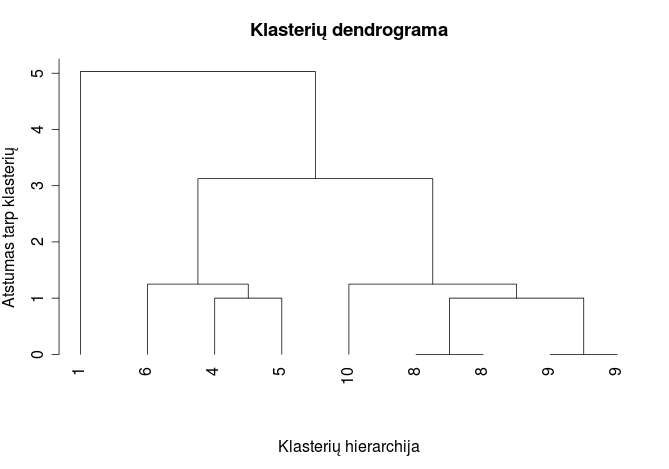
\includegraphics[width=0.6\textwidth]{images/hierarchical_clustering.png}
 \caption{Hierarchinio klasterizavimo rezultatų grafinis pavyzdys.}
 \label{fig:hierarchical_clustering}
\end{figure}
% Šio skyrelio reikia, nes Consensus Group Stable matų atrinkimo metodas naudoja hierarchinio klasterizavimo algoritmą

Hierarchinis klasterizavimas (angl. \textit{hierarchical clustering}) yra klasterizavimo algoritmas, kuris arba visą duomenų aibę panariui skaido į vis mažesnius klasterius (angl. \textit{divisive clustering}), arba pradeda nuo klasterių sudarytų tik iš vieno mėginio ir kiekvienoje iteracijoje sujungia panašiausius klasterius (angl. \textit{agglomerative clustering}) \cite{DBLP:books/mk/HanK2000}.  Hierarchinio klasterizavimo rezultatas -- klasterių medis, dendrograma, rodanti, kaip klasteriai yra hierarchiškai susiję. Pasirinktame lygyje nupjovus dendrogramą gaunama klasterizavimo struktūra \cite{martisiute08}. Klasterių dendrogramos pavyzdys yra pateiktas \ref{fig:hierarchical_clustering} pav. Hierarchinis klasterizavimas yra informatyvesnis nei paprastas -- plokščias -- klasterizavimas. Tačiau šių algoritmų sudėtingumas didesnis nei, pvz., tankiu grįstų algoritmų \cite{DBLP:books/mk/HanK2000}.

\subsection{Mokymosi su mokytoju ir mokymosi be mokytojo palyginimas}

 Mokymosi su ir be mokytojo procesai panašūs savo esme -- siekia išgauti žinias apie turimus duomenis, tačiau jų panaudojimas skiriasi iš esmės:
\begin{itemize}
  \item Mokymosi duomenys -- mokymosi su mokytoju proceso įeities duomenyse yra išreikštinai pasakyta, kokio rezultato mes laukiame, o mokymosi be mokytojo įeities duomenyse tokios papildomos informacijos nėra.
  \item  Naudojimo tikslai -- mokymasis su mokytoju siekia iš pavyzdžių išmokti vertinti naujus duomenis, o mokymasis be mokytojo siekia atrasti vidinę duomenų struktūrą.
\end{itemize}

%% JG: aš nesutinku, kad abiem procesais siekiama tųÂ pačių tikslų. Vienu atveju 
% siekiama išmokti iš pavyzdžių. Kitu atveju siekiama atrasti nežinomas
% struktūras turimuose duomenyse. Procesai yra panašūs savo esme, bet jų 
% panaudojimas skiriasi iš esmės.

%% JG: iš vikipedijos: In machine learning, unsupervised learning refers to the 
% problem of trying to find hidden structure in unlabeled data. Since the
% examples given to the learner are unlabeled, there is no error or reward
% signal to evaluate a potential solution. This distinguishes unsupervised 
% learning from supervised learning and reinforcement learning.

%% JG: visą šitą skyrių reikia pateikti koncentruotai. Esminiai teiginiai ir grafiniai pavyzdžiai. 

%% DJ: Turiu pripažint, kad šitam pavyzdyje prigrybavau stipriai. Nurašinėjau
% pavyzdį kur prastai paaiškino skirtumą, bet užtat man pavyzdys patiko. Dabar
% labiau į temą surašyta.

\subsection{Kombinuotasis mokymasis}

Kombinuotasis mokymasis (angl. \textit{ensemble learning}) - tai toks mašininis mokymasis, kai problemos sprendimui yra kombinuojami keli mašininio mokymos metodai. Pristatant kombinuotojo mokymosi principus naudojama klasifikatoriaus sąvoka, tačiau principai galioja ir kitiems mašininio mokymosi metodams, pvz., matų atrinkimui ir klasifikavimui. Kombinuotojo mokymosi metodai turi sugebėti konstruoti pavienius klasifikatorius ir kombinuoti tų klasifikatorių gautus rezultatus. Yra keletas kombinuotojo mokymosi metodų, kurių populiariausi yra \textit{bagging} \cite{breiman1996bagging}, \textit{boosting} \cite{schapire2003boosting}, \textit{stacking} \cite{wolpert1992stacked}, etc.

Kombinuotasis mokymasis pirmiausia yra naudojamas tam, kad pagerintų kuriamo klasifikatoriaus tikslumą arba sumažintų prasto klasifikatoriaus sukūrimo tikimybę, nes dažniausiai nėra žinoma, kuris klasifikavimo algoritmas ir kokia jo konfigūracija geriausiai tinka nagrinėjamai problematikai. Tipinės situacijos, kai kombinuotojo mokymosi metodų taikymas pasiteisina \cite{polikar2006ensemble}:
\begin{enumerate}
 \item Statistinis reikšmingumas -- imant keletos klasifikatorių vidutinį rezultatą, yra sumažinama rizika pasirinkti netinkamą klasifikatorių.
 \item Dideli duomenų kiekiai -- kartais duomenų būna tiek, kad juos apdoroti vienam klasifikatoriui yra labai neefektyvu, o kombinuojant keletą klasifikatorių pasiekiamas geresnis efektyvumas.
 \item Mažas mėginių skaičius -- daugelio klasifikatorių apmokymas su vis kitu mėginių poaibiu padeda tiksliau nuspėti tikrąją duomenų funkciją.
 \item Skaldyk ir valdyk -- kai kurie duomenys yra per sudėtingi, kad jie būtų išmokti vienu klasifikatoriumi. Tačiau kombinuojant keletą klasifikatorių galima išmokti net ir labai komplikuotus duomenis. 
 \item Duomenų suliejimas -- kartais duomenys gaunami iš keletos šaltinių, vienam klasifikatoriui apdoroti tokius duomenimis gali būti per sunku, todėl pasiteisina skirtingų klasifikatorių naudojimas atskiriems duomenų rinkiniams, kombinuojant jų rezultatus.
\end{enumerate}
Kombinuotasis mokymasis gali būti palygintas su keletos ekspertų apklausa, todėl kombinuotojo mokymosi metodų naudojimas sudėtingose problemose, pvz., darbas su biomedicininiais duomenimis, pasiteisina.
